%%%%%%%%%%%%%%%%%%%%%%%%%%%%%%%%%%%%%%%%%
% Programming/Coding Assignment
% LaTeX Template
%
% This template has been downloaded from:
% http://www.latextemplates.com
%
% Original author:
% Ted Pavlic (http://www.tedpavlic.com)
%
% Note:
% The \lipsum[#] commands throughout this template generate dummy text
% to fill the template out. These commands should all be removed when 
% writing assignment content.
%
% This template uses a Perl script as an example snippet of code, most other
% languages are also usable. Configure them in the "CODE INCLUSION 
% CONFIGURATION" section.
%
%%%%%%%%%%%%%%%%%%%%%%%%%%%%%%%%%%%%%%%%%

%----------------------------------------------------------------------------------------
%	PACKAGES AND OTHER DOCUMENT CONFIGURATIONS
%----------------------------------------------------------------------------------------

\documentclass{article}

\usepackage{fancyhdr} % Required for custom headers
\usepackage{lastpage} % Required to determine the last page for the footer
\usepackage{extramarks} % Required for headers and footers
\usepackage[usenames,dvipsnames]{color} % Required for custom colors
\usepackage{graphicx} % Required to insert images
\usepackage{listings} % Required for insertion of code
\usepackage{courier} % Required for the courier font
\usepackage{lipsum} % Used for inserting dummy 'Lorem ipsum' text into the template
\usepackage[utf8]{inputenc} % Required for inputting international characters
\usepackage[T1]{fontenc} % Output font encoding for international characters
\usepackage{pdfpages}

% Margins
\topmargin=-0.45in
\evensidemargin=0in
\oddsidemargin=0in
\textwidth=6.5in
\textheight=9.0in
\headsep=0.25in

\linespread{1.1} % Line spacing

% Set up the header and footer
\pagestyle{fancy}
\lhead{\hmwkTitle} % Top left header
\rhead{\hmwkAuthorName} % Top right header
%\chead{\hmwkClass\ (\hmwkClassInstructor\ \hmwkClassTime): \hmwkTitle} % Top center head
%\rhead{\firstxmark} % Top right header
\lfoot{\lastxmark} % Bottom left footer
\cfoot{} % Bottom center footer
\rfoot{Strana\ \thepage\ - \protect\pageref{LastPage}} % Bottom right footer
\renewcommand\headrulewidth{0.4pt} % Size of the header rule
\renewcommand\footrulewidth{0.4pt} % Size of the footer rule

\setlength\parindent{0pt} % Removes all indentation from paragraphs

%----------------------------------------------------------------------------------------
%	CODE INCLUSION CONFIGURATION
%----------------------------------------------------------------------------------------

\definecolor{MyDarkGreen}{rgb}{0.0,0.4,0.0} % This is the color used for comments
\lstloadlanguages{C++} % Load C++ syntax for listings
\lstset{language=C++, % Use c++ in this example
        frame=single, % Single frame around code
        basicstyle=\small\ttfamily, % Use small true type font
        keywordstyle=[1]\color{Blue}\bf, % c++ functions bold and blue
        keywordstyle=[2]\color{Purple}, % c++ function arguments purple
        keywordstyle=[3]\color{Blue}\underbar, % Custom functions underlined and blue
        identifierstyle=, % Nothing special about identifiers                                         
        commentstyle=\usefont{T1}{pcr}{m}{sl}\color{MyDarkGreen}\small, % Comments small dark green courier font
        stringstyle=\color{Purple}, % Strings are purple
        showstringspaces=false, % Don't put marks in string spaces
        tabsize=5, % 5 spaces per tab
        %
        % Put standard c++ functions not included in the default language here
        morekeywords={rand},
        %
        % Put c++ function parameters here
        morekeywords=[2]{on, off, interp},
        %
        % Put user defined functions here
        morekeywords=[3]{test},
       	%
        morecomment=[l][\color{Blue}]{...}, % Line continuation (...) like blue comment
        numbers=left, % Line numbers on left
        firstnumber=1, % Line numbers start with line 1
        numberstyle=\tiny\color{Blue}, % Line numbers are blue and small
        stepnumber=5 % Line numbers go in steps of 5
}

% Creates a new command to include a perl script, the first parameter is the filename of the script (without .pl), the second parameter is the caption
\newcommand{\perlscript}[2]{
\begin{itemize}
\item[]\lstinputlisting[caption=#2,label=#1]{#1.pl}
\end{itemize}
}

%----------------------------------------------------------------------------------------
%	DOCUMENT STRUCTURE COMMANDS
%	Skip this unless you know what you're doing
%----------------------------------------------------------------------------------------

% Header and footer for when a page split occurs within a problem environment
\newcommand{\enterProblemHeader}[1]{
\nobreak\extramarks{#1}{#1 pokračování na další straně\ldots}\nobreak
\nobreak\extramarks{#1 (pokračování)}{#1 pokračování na další straně\ldots}\nobreak
}

% Header and footer for when a page split occurs between problem environments
\newcommand{\exitProblemHeader}[1]{
\nobreak\extramarks{#1 (pokračování)}{#1 pokračování na další straně\ldots}\nobreak
\nobreak\extramarks{#1}{}\nobreak
}

%----------------------------------------------------------------------------------------
%	NAME AND CLASS SECTION
%----------------------------------------------------------------------------------------

\newcommand{\hmwkTitle}{Geometrické vyhledávání bodu} % Assignment title
\newcommand{\hmwkDueDate}{Datum odevzdání: 13.11.2017} % Due date
\newcommand{\hmwkClass}{155ADKG} % Course/class
%\newcommand{\hmwkClassTime}{10:30am} % Class/lecture time
%\newcommand{\hmwkClassInstructor}{Jones} % Teacher/lecturer
\newcommand{\hmwkAuthorName}{Petra~Millarová, Bc.~Oleksiy~Maybrodskyy} % Your name

%----------------------------------------------------------------------------------------
%	TITLE PAGE
%----------------------------------------------------------------------------------------

\title{
\vspace{2in}
\textmd{\textbf{\hmwkClass:\ \hmwkTitle}}\\
\normalsize\vspace{0.1in}\large{\hmwkDueDate}\\
%\vspace{0.1in}\large{\textit{\hmwkClassInstructor\ \hmwkClassTime}}
\vspace{3in}
}

\author{\textbf{\hmwkAuthorName}}
\date{} % Insert date here if you want it to appear below your name

%----------------------------------------------------------------------------------------

\begin{document}

\maketitle

%----------------------------------------------------------------------------------------
%	TABLE OF CONTENTS
%----------------------------------------------------------------------------------------

%\setcounter{tocdepth}{1} % Uncomment this line if you don't want subsections listed in the ToC

\newpage
\tableofcontents
\newpage

%----------------------------------------------------------------------------------------
%	PROBLEM 1
%----------------------------------------------------------------------------------------

% To have just one problem per page, simply put a \clearpage after each problem

\section{Zadání}
\indent Následuje kopie oficiálního zadání úlohy. Autoři z nepovinných bodů zadání implementovali všechny kromě algoritmu pro automatcké generování nekonvexních polygonů.
\begin{figure}[htbp]
    \centering
        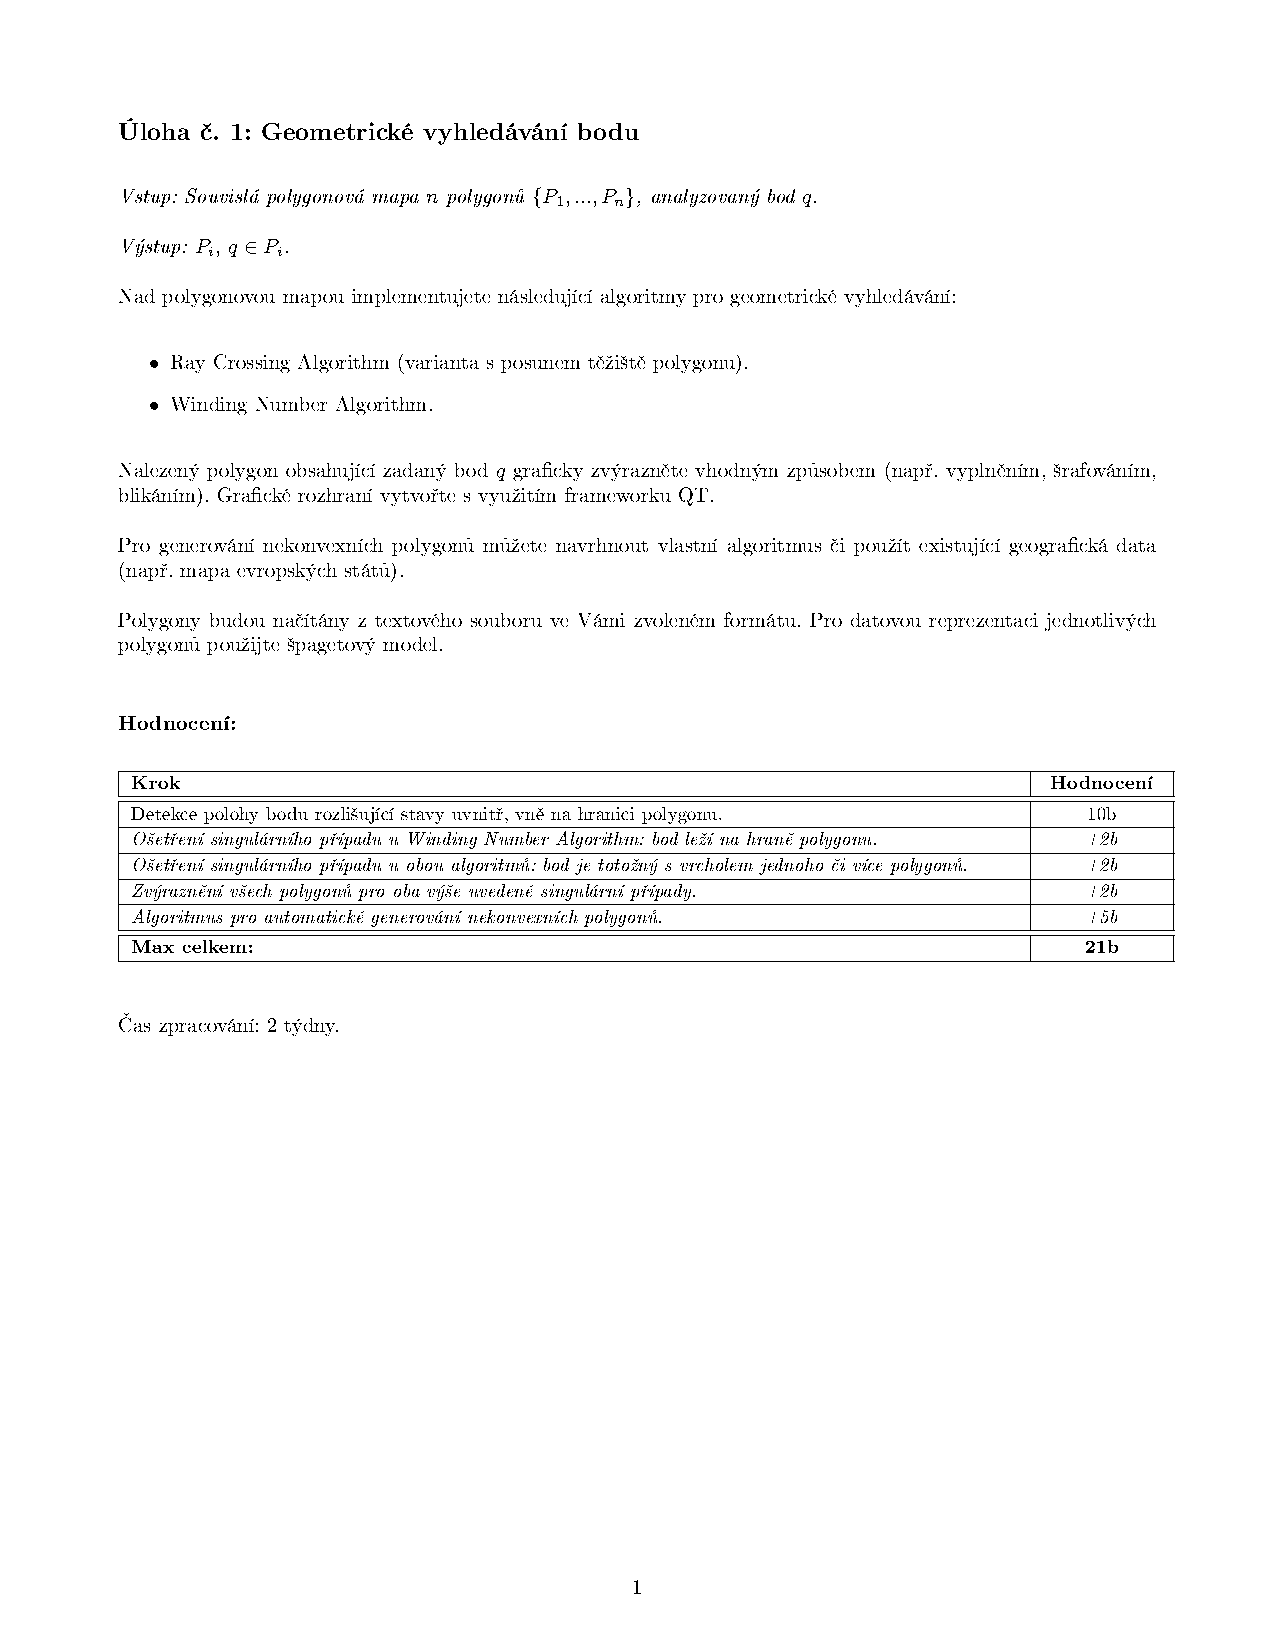
\includegraphics[clip, trim=0cm 11cm 0cm 0cm, width=1.00\textwidth]{zadani.pdf}
\end{figure}
\clearpage
\section{Popis a rozbor problému} %+vzorce
\indent 
Tato úloha se věnuje řešení praktického problému určování pozice uživatelem zadaného bodu $q$ vůči polygonům načteným ze souboru. Jako implementaci si lze zjednodušeně představit zjišťování polohy konkrétního bodu kliknutím na digitální mapě. 
\\
\\
\textsl{Nechť existuje pole ve dvojrozměrné kartézské soustavě s \textbf n body. Uzavřením tohoto pole vznikne polygon. Polygon může nabývat jak konvexní, tak nekonvexní tvar.}
\\
\\
Polygon je konvexní právě tehdy, když poloha všech bodů je vůči jakékoliv přímce procházející vedle polygonu, vždy na stejné straně. 

Rozdíl mezi \textsl konvexním a  \textsl nekonvexním polygonem je možné názorně vidět na obrázcích níže.
\begin{figure}[htbp]
\centering
        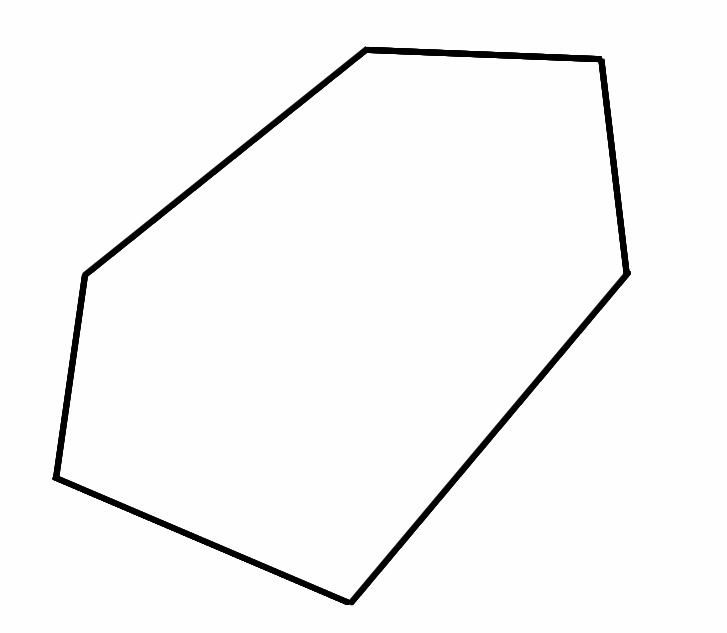
\includegraphics[clip, trim=0cm 0cm 0cm 0cm, width=0.2500\textwidth]{obrazek1.png}
 
\includegraphics[clip, trim=0cm 0cm 0cm 0cm, width=0.2500\textwidth]{obrazek2.png}
\end{figure}
\bigskip
\begin{center}
obr 1.:\textsl{konvexní polygon (vlevo) a nekonvexní polygon (vpravo)}
\end{center}
Pokud následně polygon rozdělíme na menší polygonové útvary, pak polohu zvoleného bodu $q$ můžeme popsat následovně: 
\begin{enumerate}
\item   Bod $q$ se nachází uvnitř polygonu  $q {\in} P_i$ 
\item   Bod $q$ se nachází vně všech polygonů  $q {\not \in} P_i$ 
\item   Bod se nachází na hraně jednoho  $q {\not \in} P_i$ nebo dvou polygonů $q {\in} P_{i,i+1}$ 
\item   Bod je totožný s vrcholem jednoho polygonu nebo více polygonů $q {\in} P_{i,i+1,...,i+n}$
\end{enumerate}
Výpočet se bude provádět na základě metod \textbf {Ray Crossing algorithm} a  \textbf {Winding Number algorithm}. Jejich výpočet je popsán v následujících kapitolách. 
\\
\clearpage
\section{Popisy algoritmů} %formálním jazykem
V dané úloze jsou použity následující algoritmy, avšak existují i další možnosti, jak polohu bodu určit (metoda pásů, Line Sweep algorithm aj.)
\subsection{Ray crossing algorithm}
\textsl{Nechť existuje uzavřený polygon ve dvojrozměrné kartézské soustavě, tvořený \textbf n body. Nechť následně existuje bod q, kteréhož polohu se snažime určit. Proložíme-li bodem q nekonečný počet paprsků směrem k polygonu, pak pro jednotlivý paprsek nastane jedna z následujících situací: }
\begin{enumerate}
\item   počet průsečíků paprsku  $k$ je roven sudému počtu, pak se bod $q$ nachází vně polygonu  $q {\not \in} P_i$ 
\item  počet průsečíků paprsku  $k$ je roven lichému počtu, pak se bod $q$ nachází uvnitř polygonu  $q \in P_i$
\end{enumerate} 
Zároveň mohou nastat singularity, respektive jisté situace, kdy algoritmus "nefunguje" a nedokáže přímo nalézt správný výsledek. V algoritmu ray crossing se konkrétně jedná o tyto případy:
\begin{enumerate}
\item   Bod se nachází na hraně jednoho  $q {\in} P_i$ nebo dvou polygonů $q {\in} P_{i,i+1}$ 
\item   Bod je totožný s vrcholem jednoho polygonu nebo více polygonů $q {\in} P_{i,i+1,...,i+n}$
\end{enumerate} 
Řešením je posun, respektive redukce vrcholů polygonů směrem k poloze bodu  $q$.
\\
Hledáný algoritmus je možné popsat následovně:
\begin{enumerate} 

\item Inicializace bodů polygonu $p_i$, počet průsečíku = 0;

\item Redukce souřadnic $x$ bodů polygonu k bodu $q$,  respektivě k paprskovému segmentu, $x_i^{'} = x_i - x_q$. 

\item  Redukce souřadnic $y$ bodů polygonu k bodu $q$, respektivě k paprskovému segmentu, $y_i^{'} = y_i - y_q$. 

\item Znovu pro ostatní body daného polygonu $p_i$/ 

\item if $(y_{i}^{'} <= 0)\&\&(y_i+1^{'} > 0)\|(y_{i}^{'} > 0)\&\&(y_i+1^{'} <= 0)$. 

\item $x_m^{'} = (x_i+1^{'}y_{i}^{'}-x_{i}^{'}y_i+1^{'})/(y_{i+1}^{'}-y_{i}^{'})$. 

\item Sčítaní počtu redukováných bodů, pro $x_i^{'} > 0$  


\item Poté nastáva situace, že pokud počet průsečíku je sudý, pak $q \in P$, pokud není, pak  $q \notin P$ 

\end{enumerate} 
\clearpage
\newpage 

\subsection{Winding Number Algorithm} 
\textsl{Nechť existuje uzavřený polygon ve dvojrozměrné kartézské soustavě, tvořený pomocí \textbf n bodů. Nechť následně existuje bod q, polohu kterého se snažíme určit. Z pohledu bodu $q$ provedeme orientaci směru ze které pak následně se určí součet všech úhlů na jednotlivé body uvedeného polygonu.}
\\
\\
Součtový úhel bude dále uváděn jako $w$. Výpočet je lepší provádět proti směru pohybu hodinových ručiček, jelikož v případě toho směru hodnota počítaných oběhů Winding Number $\Omega$  dosahuje kladných hodnot. Je třeba taky pamatovat, že hodnota $\Omega$ je uváděna v počtech oběhů a je záporná při oběhu ve směru 
hodinových ručiček a kladná ve směru opačném. Do výpočtu taky vstupuje tolerance $\epsilon$, která zahrnuje vlivy v zaokrouhlování. Dle uvedené matematické podmínky, může nastát následující výsledky:
\begin{enumerate} 
\item $w$=\textbf {2R}, pak $q \in P_i$ 
\item  $w$ < \textbf {2R}, pak $q {\not \in} P_i$
\end{enumerate}
 Níže je uveden algoritmus výpočtu: 

\begin{enumerate} 

\item Vstup $\omega = 0$, tolerance $\epsilon$

\item Orientace z bodu $q$ káždého následujícího bodu  $p_{i+1}$ od orientaci na bod $p_i$

\item Určení úhlu $\omega_i = \angle p_i, q, p_{i+1}$ 

\item  $\omega = \omega + \omega_i$, pro bod vprávo od orientace na bod $p_i$, pokud bod vlevo od orientace na bod $p_i$, pak $\omega = \omega - \omega_i$

\item Pokud platí podmínka $(\left|\omega - 2\Pi \right| < \epsilon)$, pak $q \in P$

\item Pokud neplatí podmínka  $(\left|\omega - 2\Pi \right| < \epsilon)$, pak $q \notin P$

\end{enumerate} 
\clearpage
\newpage
\section{Problematické situace a singularity} %rozbor a osetreni v kodu
\clearpage
\section{Vstupní data}
\clearpage
\subsection{Formát vstupních dat}
\clearpage
\subsection{Popis dat}
\clearpage
\section{Výstupní data}
	\subsection{Formát výstupních dat}
	\subsection{Popis dat}
\clearpage
\section{Ukázka aplikace} %printscreen
\clearpage
\section{Závěr}
	\subsection{Náměty na vylepšení} %+možné či neřešené problémy
\bibliography{u1}
\bibliographystyle{plain}
\addcontentsline{toc}{section}{References}
\pagestyle{empty}

%\end{homeworkSection}
\clearpage

%-----------------------------------------------------------------------------
\end{document}